\section{Elaborando pruebas de una aplicación Web} 
\begin{itemize}
 \item  Crear el proyecto de prueba de .NET Core.
\begin{center}
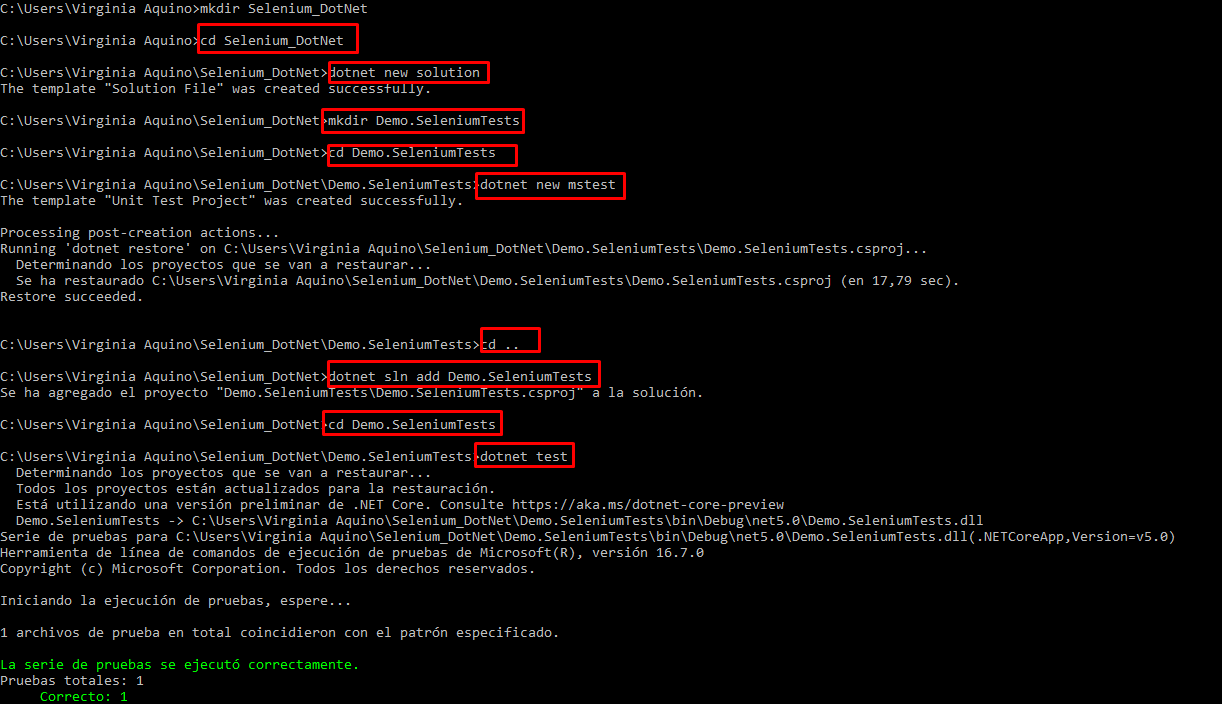
\includegraphics[width=\columnwidth]{images/1}\newline
\end{center}
\item Agregue Selenium al proyecto de prueba 
\begin{center}
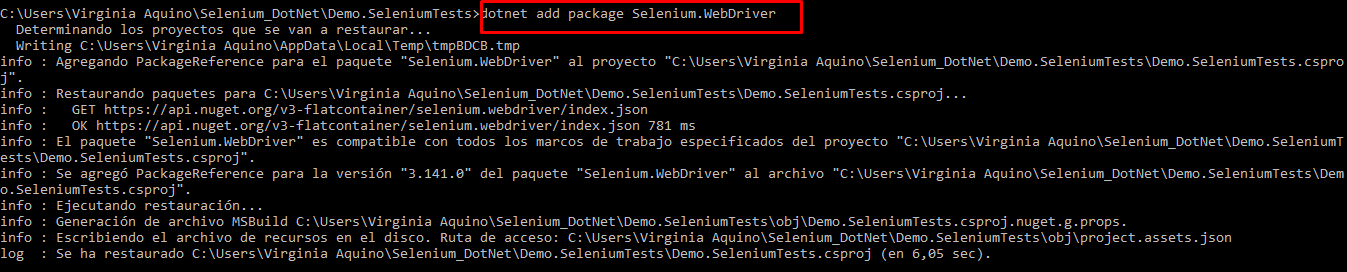
\includegraphics[width=\columnwidth]{images/2}\newline
\end{center}
\item Escriba una prueba de IU usando Selenium
\begin{center}
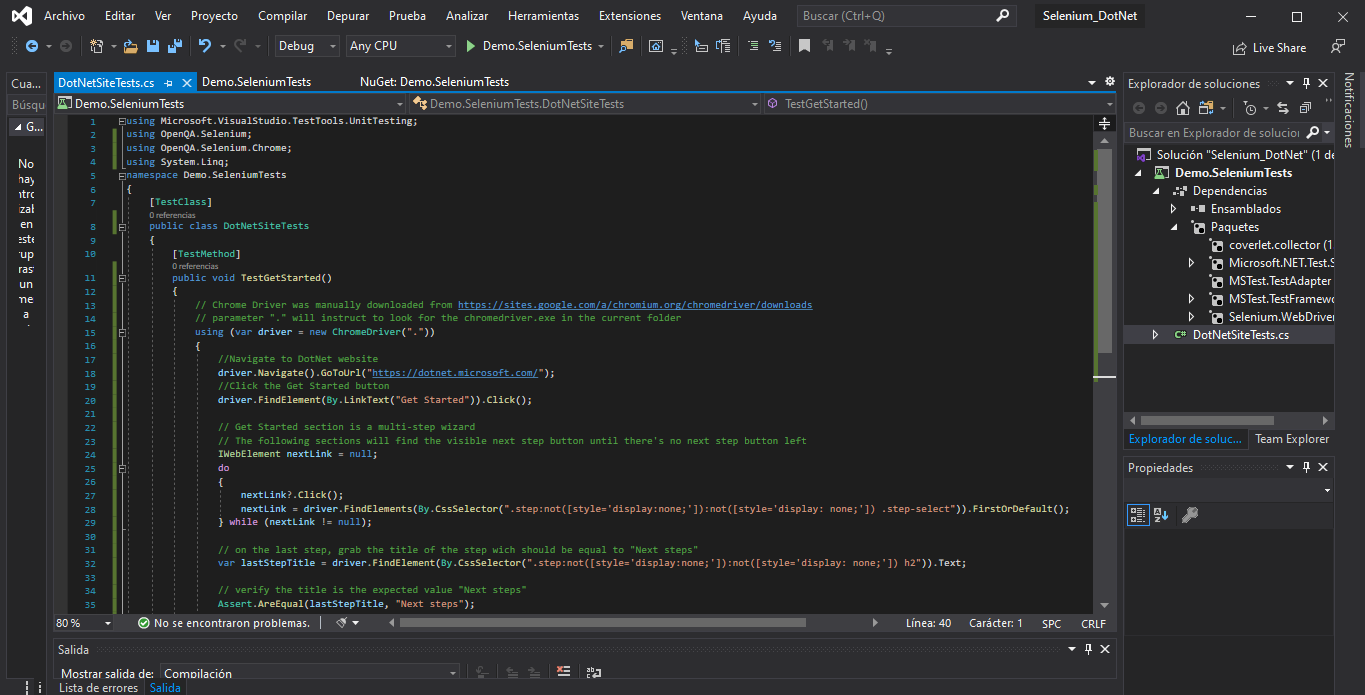
\includegraphics[width=\columnwidth]{images/3}\newline
\end{center}
\item Ejecute la prueba de IU
\begin{center}
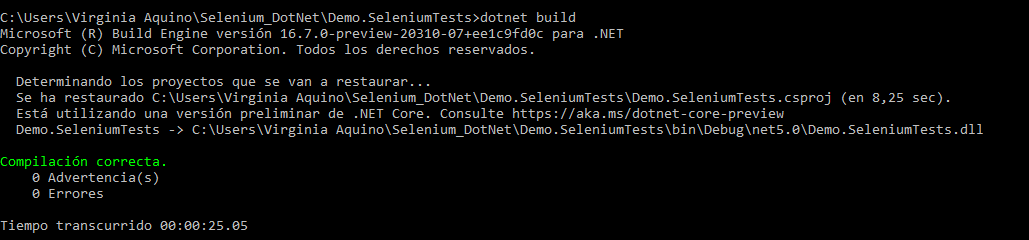
\includegraphics[width=\columnwidth]{images/4}\newline
\end{center}
\item Para Windows, puede usar este script de PowerShell:
\begin{center}
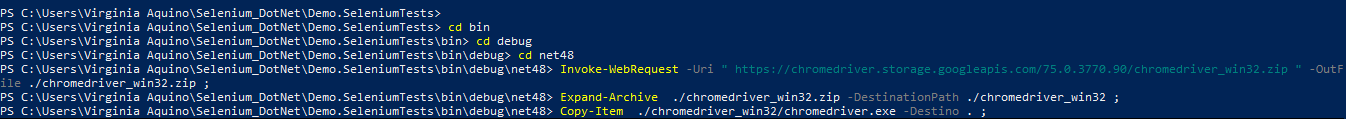
\includegraphics[width=\columnwidth]{images/5}\newline

\includegraphics[width=\columnwidth]{images/6}\newline
\end{center}
\item Solución de problemas: si la prueba falla debido a errores de Chrome / Chromium, siga estos pasos
Asegúrese de tener instalado Chrome / Chromium. descargar chrome version 75
\begin{center}
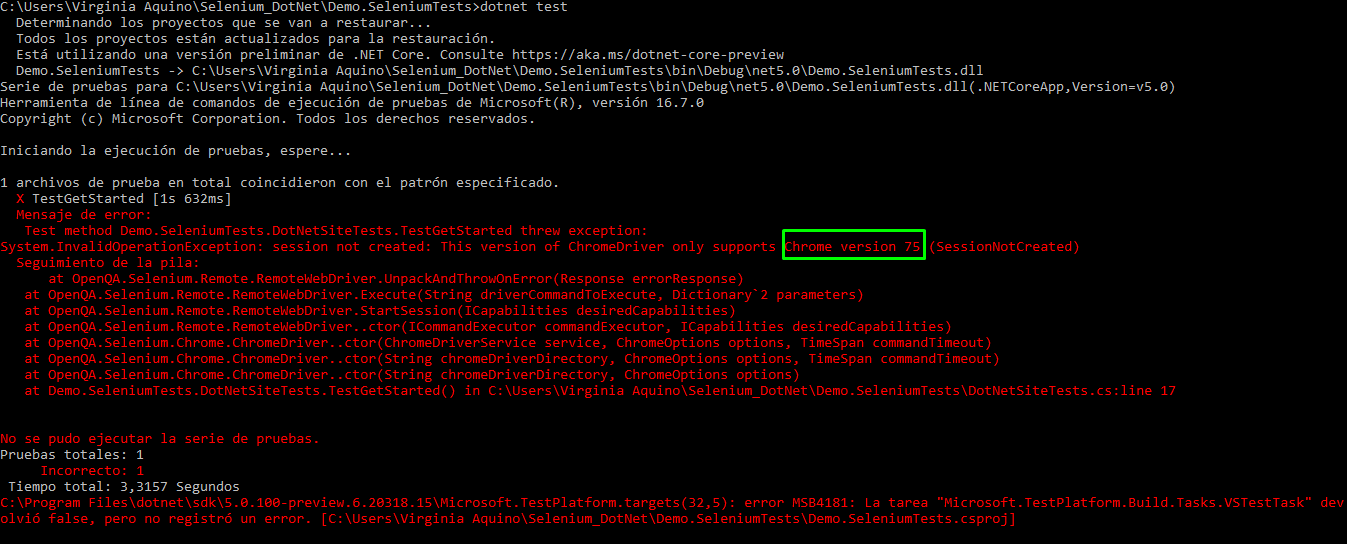
\includegraphics[width=\columnwidth]{images/error}\newline
\end{center}
\item Ejecute el comando de prueba dotnet
\begin{center}
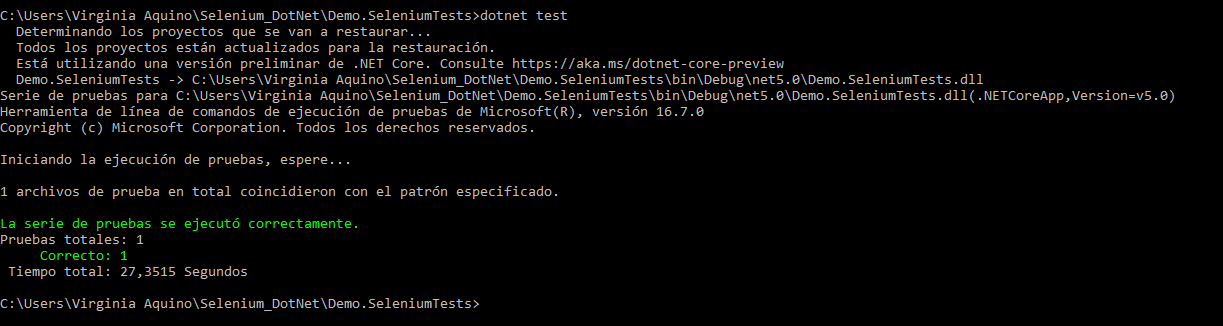
\includegraphics[width=\columnwidth]{images/final}\newline
\end{center}
\end{itemize}
